\chapter{Day 3: conditionals \& interactivity}

\section{Summary of topics}
% Summarize the topics from the “listen” segment of the day (150 – 250 words)

In the lesson of today we continued with conditionals. The \texttt{else} keyword was again explained, after which we also learned about the \texttt{else if} keyword. Expanding upon example 2.3 from yesterday we get:

\begin{codebox}{example 3.1}
    \begin{lstlisting}
if (relational expression 1) {
    // lines to be executed if expression 1 is true
} else if (relation expression 2) {
    // lines to be executed if expression 2 is true
} else {
    // lines to be executed if both expression 1 and 2 are false
}
    \end{lstlisting}
\end{codebox}

Next, logical operators where demonstrated. These allow you to combine multiple relational expression together into a single relational expression. These are as follows:

\begin{codebox}{example 3.2}
    \begin{lstlisting}
expr 1 && expr 2 // Expr 1 and 2 need to be true to return true
expr 1 || expr 2 // Expr 1 and/or 2 need to be true to return true
!expr 1 // Expr 1 needs to be false to return true and vice versa
    \end{lstlisting}
\end{codebox}

The next topic was about user interaction. First the variables \texttt{mouseX} and \texttt{mouseY} of yesterday were explained again. Next, two methods to detect mouse button presses and key presses where demonstrated. The first method uses the \texttt{keyPressed} and \texttt{mousePressed} variables. If a key or mouse button is pressed, the respective variable returns \texttt{true}. Then, with the variables \texttt{key} and \texttt{mouseButton}, you can read out which key or button was pressed. See the code examples below.

\begin{codebox}{example 3.3}
    \begin{lstlisting}
if (keyPressed) { // check if a key was pressed
    if (key == 'w') {
        // this code is executed when the 'w' key is pressed
    } 
}
    \end{lstlisting}
\end{codebox}

\newpage

\begin{codebox}{example 3.4}
    \begin{lstlisting}
if (mousePressed) { // check if a mouse button was pressed
    if (mouseButton == LEFT) {
        // this code is executed when the left mouse button is pressed
    } 
}
    \end{lstlisting}
\end{codebox}

The disadvantage of this first method is that the program is not interrupted when the user presses a key. If the main loop of the program takes a long time, a key press might be missed. The second method uses events, which interrupt the program if the conditions for that event are met (like pressing a button). A event triggers a method which is then executed once. Examples of mouse Events are \texttt{mousePressed()}, \texttt{mouseReleased()} and \texttt{mouseMoved()}. Examples of key events are \texttt{keyPressed()} and \texttt{keyReleased()}. In all these methods you can use the variables \texttt{key} and \texttt{mouseButton} similarly to example 3.3 and 3.4 to detect which key or button was pressed.

\section{Challenge description: Give Me Space}
% A description of that day’s challenge describing what the assignment was, what you tried to achieve and how you applied the topics from the “listen” segment. include instruction on how to use is and Include screenshots/screen captures. (150 – 250 words)

Today's goal was to create a simple game with a clear winning and/or losing condition. I created a game called \textit{Give Me Space}. The game is loosely inspired by arcade games like \textit{Space Invaders} and \textit{breakout}. The goal is to survive as long as possible, while destroying any asteroids that come on your path.

The game is shown in \cref{fig: give me space}. When launching the game a start screen is shown with the current highscore. You can press space (a joke I was quite pleased with) to start the game (\cref{fig: space new game}). The game is played using W, A and D. W moves the spaceship forward, and A and D rotate the spaceship. The mouse can be used to aim, with left click shooting a bullet. Asteroids require 1-3 bullets to be destroyed, earing 100 points. Every few seconds an extra 150 points are rewarded. When you get hit by an asteroid, you loose some health (\cref{fig: space game}). One can pause and unpause the game at any moment by pressing the space key (\cref{fig: space paused game}). The game is over when your health reaches 0. The score is shown and one can press the space again to go back to the main menu (\cref{fig: space game over}).

\begin{figure}[H]
    \centering
    \begin{subfigure}[b]{0.45\textwidth}
        \centering
        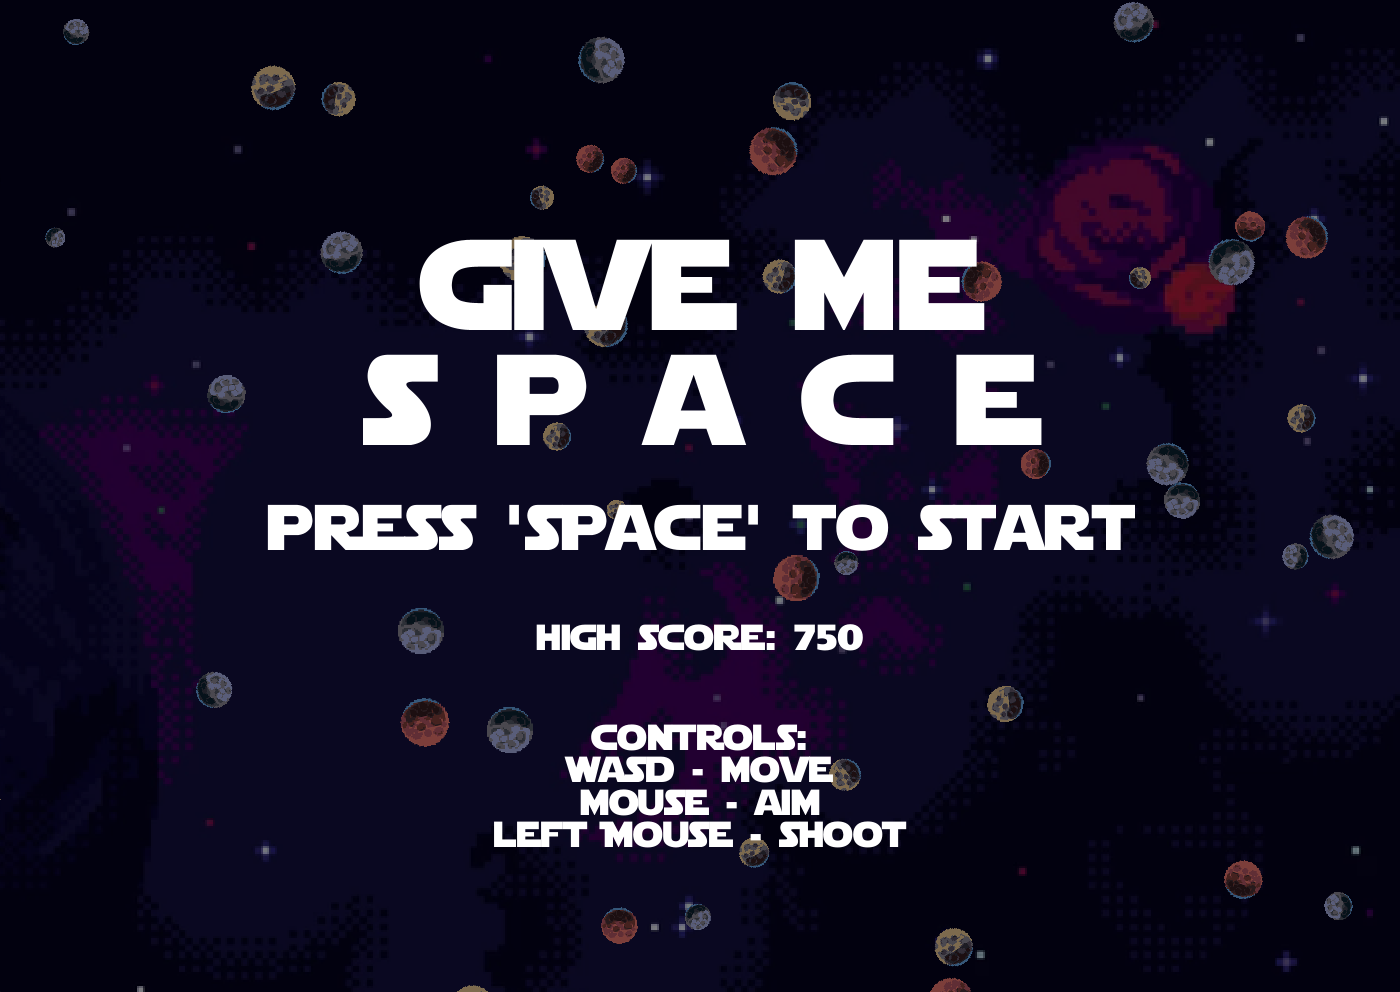
\includegraphics[width=\textwidth]{Figures/day_3/menu.png}
        \caption{Starting a new game}
        \label{fig: space new game}
    \end{subfigure}
    \hspace{1cm}
    \begin{subfigure}[b]{0.45\textwidth}
        \centering
        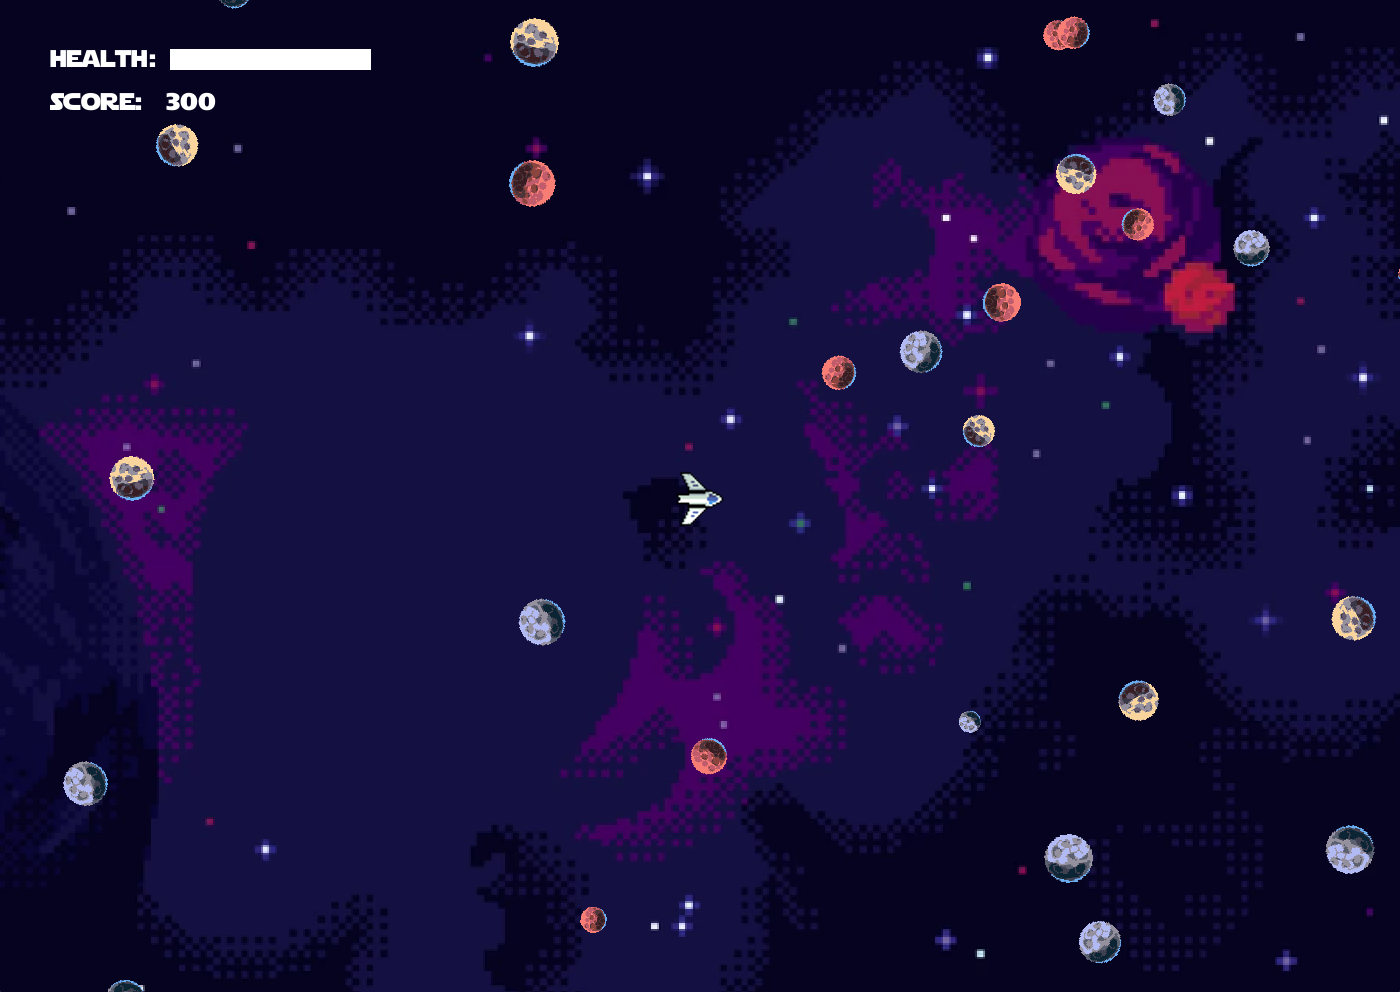
\includegraphics[width=\textwidth]{Figures/day_3/game.png}
        \caption{Playing the game}
        \label{fig: space game}
    \end{subfigure}
    \label{fig: give me space}

\end{figure}

\begin{figure}[H]
    \ContinuedFloat
    \centering
    \begin{subfigure}[b]{0.45\textwidth}
        \centering
        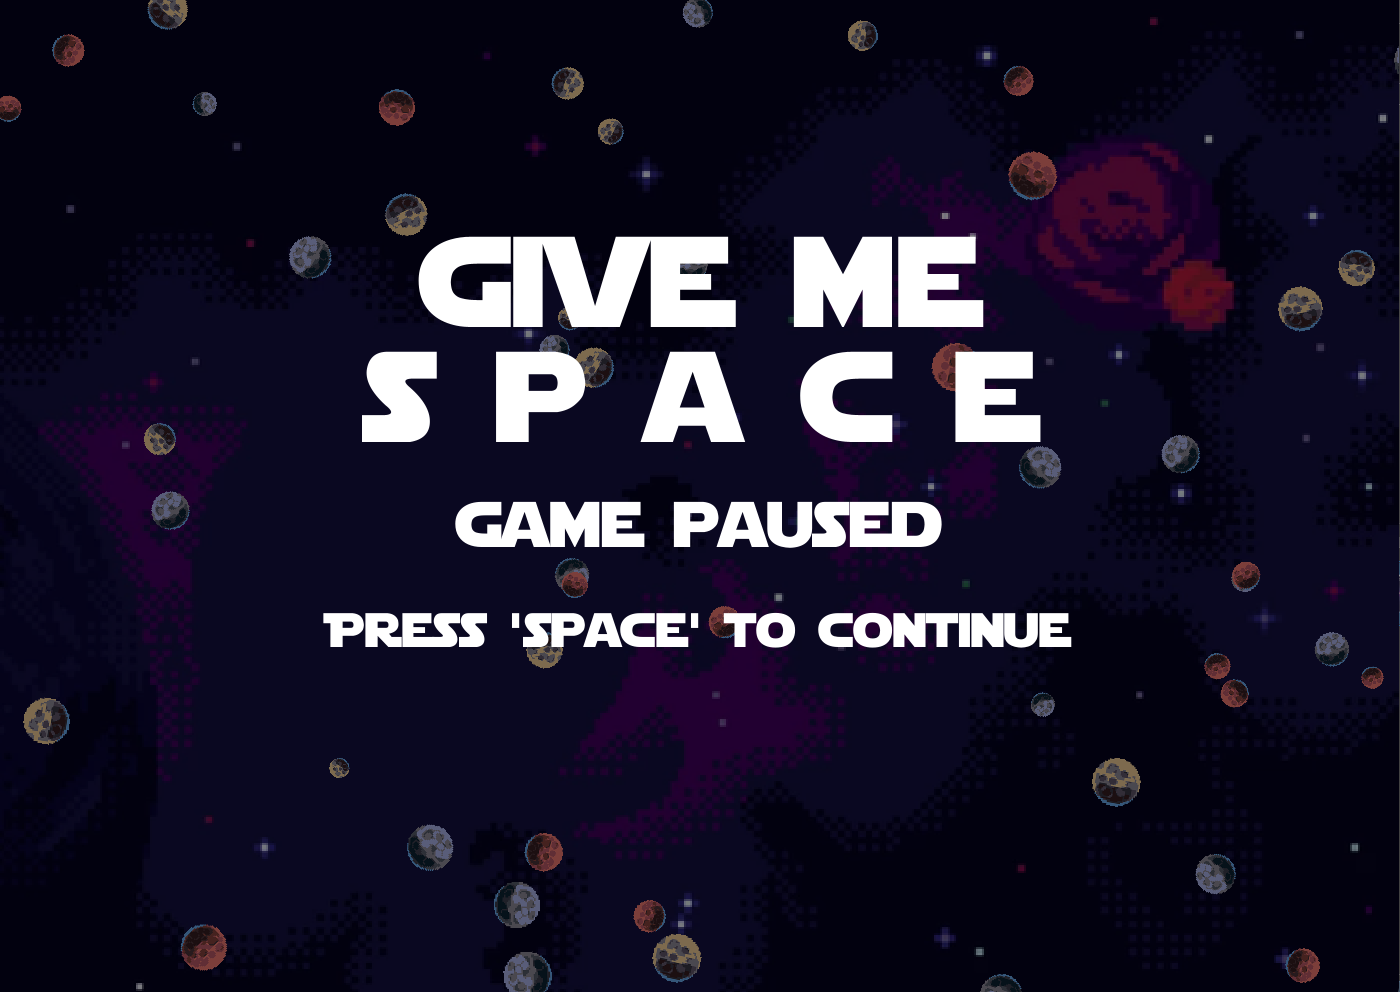
\includegraphics[width=\textwidth]{Figures/day_3/paused.png}
        \caption{Pausing the game}
        \label{fig: space paused game}
    \end{subfigure}
    \hspace{1cm}
    \begin{subfigure}[b]{0.45\textwidth}
        \centering
        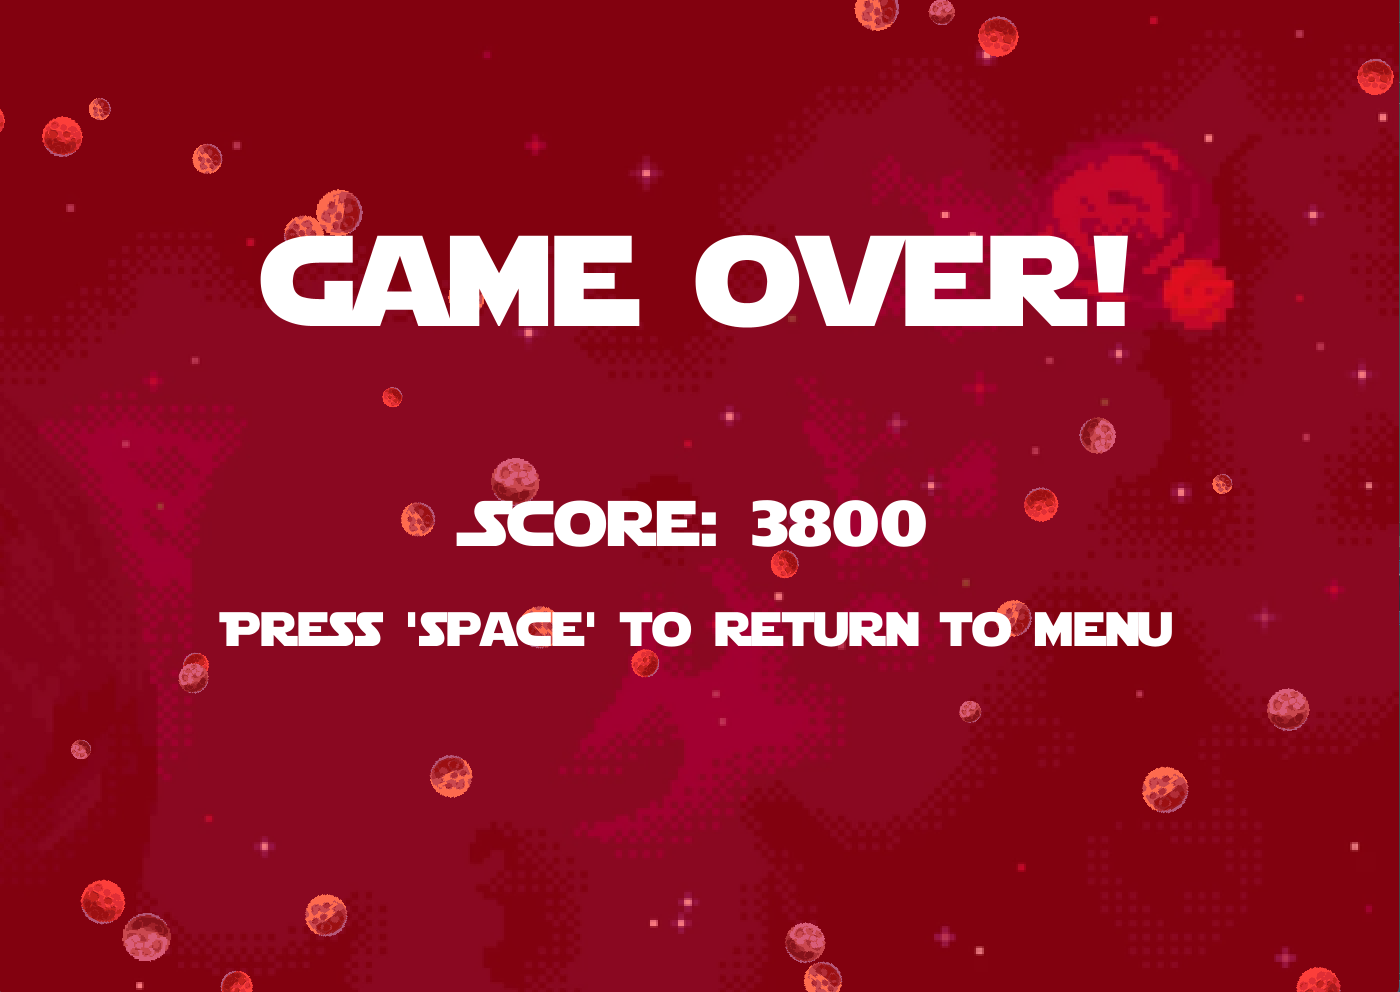
\includegraphics[width=\textwidth]{Figures/day_3/game_over.png}
        \caption{Game over}
        \label{fig: space game over}
    \end{subfigure}

    \caption{A typical game of Give Me Space (continued)}

\end{figure}

The game uses if-statements on plenty of occasions, like to check if the bullets or asteroids are of the screen and should be removed, or during the collision detection. User input is received using the \texttt{keyPressed()} and \texttt{mousePressed()} methods and the \texttt{key} and \texttt{mouseX}/\texttt{mouseY} variables. Finally, The \texttt{setup()} and \texttt{draw()} methods are used to animate the game.